% ABLS - term-long paper

\documentclass{sig-alternate}

\usepackage{url}
\usepackage{color}
\usepackage{enumerate}
\usepackage{balance}
\usepackage{verbatim}
\usepackage{enumitem}
\usepackage[table]{xcolor}
\usepackage{multicol,multirow}
\usepackage{subfig}
\usepackage{dcolumn}
\usepackage{palatino}
\usepackage{bbm}
\usepackage{url}
\usepackage{verbatim}
\usepackage{algorithm}
\usepackage[noend]{algorithmic}
\usepackage{fancybox, fancyvrb}
\usepackage{listings}

\permission{}
\CopyrightYear{2012}
%\crdata{0-00000-00-0/00/00}
\begin{document}

\title{ABLS - An Attribute Based Logging System for the Cloud}
\numberofauthors{1}
\author{
\alignauthor{
Christopher A. Wood \\
Department of Computer Science \\
{\tt caw4567@rit.edu}
}}
\date{\today}
\maketitle
\begin{abstract}
User-based non-repudiation is an increasingly important property of cloud-based applications. It provides irrefutable evidence that ties system behavior to specific users, which in turn enables the strict enforcement of organizational security policies. System logs, which can be used to construct audit trails, are typically used as the basis for this property. Thus, the effectiveness of system audits based on log files reduces to the problem of maintaining the integrity and confidentiality of log files. We present the design and implementation of an attribute-based logging system, ABLS, that is capable of building secure log files. In doing so, we also present some of the benefits of ciphertext-policy attribute-based encryption (CP-ABE) to solve a variety of log design issues. In addition, we also present the design of an automated auditing procedure
that is dynamically configurable by its users to aid in security policy enforcement.
\end{abstract}

\section{Introduction}
User-based non-repudiation is a system security property that provides indisputable evidence linking
specific actions to individual users (or entities) that trigger such actions. Cryptographically speaking, 
non-repudiation requires that the integrity and 
origin of all data should be provable. In essence, this enables system audits to be conducted that can
identify data misuse, and thus, potential security policy violations, by comparing the contextual information 
of system events (e.g. source user, time of the event, etc) with all entities authorized to invoke such events. 
Therefore, treating non-repudiation as a required system quality attribute in the architecture is likely to 
become a common trend in the commercial, government, and even more specifically, the health-care domain.

System audits typically use log files to determine the ``who, what, when, and how'' of events that took 
place during the system's lifetime. In order to provide accurate information for non-repudiation purposes,
it is often necessary to place some amount user-sensitive data in these log files that can be used
to trace data back to its origin. As such, logs of events generated by a client that is being served must
maintain data confidentiality and integrity should the system be compromised. These goals are commonly achieved
using a combination of encryption and signature techniques \cite{Ma2008-FssAgg}. However, traditional approaches to
encryption and signature generation and verification are becoming less effective in the context of cloud
applications. Similarly, naive approaches to log security that are based on tamper-resistant hardware and 
maintaining continuous secure communication channels between a log aggregator and end user are less applicable in 
the context of cloud-based applications \cite{Schneier1999-Secure}. 

Symmetric-key and public-key encryption of log entries are very common confidentiality techniques 
proposed in the literature. Unfortunately, these schemes are becoming less useful in cloud-based applications.
There is a need for robust access control mechanisms that enable dynamic user addition and revocation
with minimal overhead. In other words, continuously re-encrypting a subset of the log database should be avoided. 
Both symmetric- and public-key cryptosystems suffer in that access policies must be tied directly to keys used for
encryption and decryption. If the access policy for a set of log messages needs to be changed, then both the keys used to
encrypt and decrypt such log entries will need to be regenerated and distributed, and the entries must also
be re-encrypted. Both of these tasks can be very expensive. 

In addition, symmetric-key cryptosystems require keys to be shared among users who need access to the 
same set of logs. This requires a secure and comprehensive key management and distribution scheme and
supporting policy. In a similar vein, public-key cryptosystems (e.g. RSA and ElGamal) suffer 
from the extra data transfer and storage requirements for large cryptographic keys and certificates. There 
may be insufficient resources to maintain a public-key infrastructure (PKI) for managing keys and digital 
certificates for all users. 

In terms of log file integrity, aggregate signature schemes that support forward secrecy through the use of 
symmetric- and public-key cryptosystems are also becoming outdated \cite{Yavuz2009-BAF}. 
Symmetric-key schemes may promote high computational efficiency for signature generation, but they 
do not directly support public verifiability for administrators and auditors. This means that robust key 
distribution schemes or the introduction of a trusted third party (TTP) are needed to ensure all required parties 
can access the necessary log information. Such schemes also 
suffer from high storage requirements and communication overhead. Public-key schemes have similar issues, 
as the increased key size leads to even larger storage requirements and less computational efficiency. 

Collectively, we see that a balance between encryption and signature generation and verification performance is
needed to support the unique scalability and resource usage requirements for cloud-based applications.
Attribute-based encryption (ABE), a new cryptographic scheme that uses user attributes (or roles, in certain 
circumstances) to maintain the confidentiality of user-sensitive data, has an appealing application
to logging systems maintained in the cloud and is capable of satisfying the aforementioned confidentiality 
requirements. From an integrity perspective, authenticated hash-chains have been shown to be effective 
at ensuring log file integrity in numerous logging schemes  \cite{Schneier1999-Secure}. 

In this paper we discuss ABLS, an attribute-based logging system that supports ciphertext-policy 
attribute-based encryption (CP-ABE) \cite{Bethencourt2007-CPABE} and authenticated hash-chain 
constructions for log file confidentiality and integrity, respectively. ABLS was designed for
the cloud and is capable of addressing the aforementioned problems with secure logging. 
We first start with the implementation highlights that were completed in Phase 1 of the project. We then
conclude with a discussion of the current status of the project and planned work to be completed.

\section{Prototype Implementation}
A proof-of-concept system has been developed in order to test both the correctness and performance of ABLS. 
In this section we provide some highlights of the prototype implementation.

\subsection{Deployment}
\label{sec:deployment}
ABLS is designed to be a centralized logging system backed by a set of distributed databases. A context
diagram for the ABLS deployment scheme is shown in Figure \ref{fig:deployment}.

\begin{figure*}[htb!]
\begin{center}
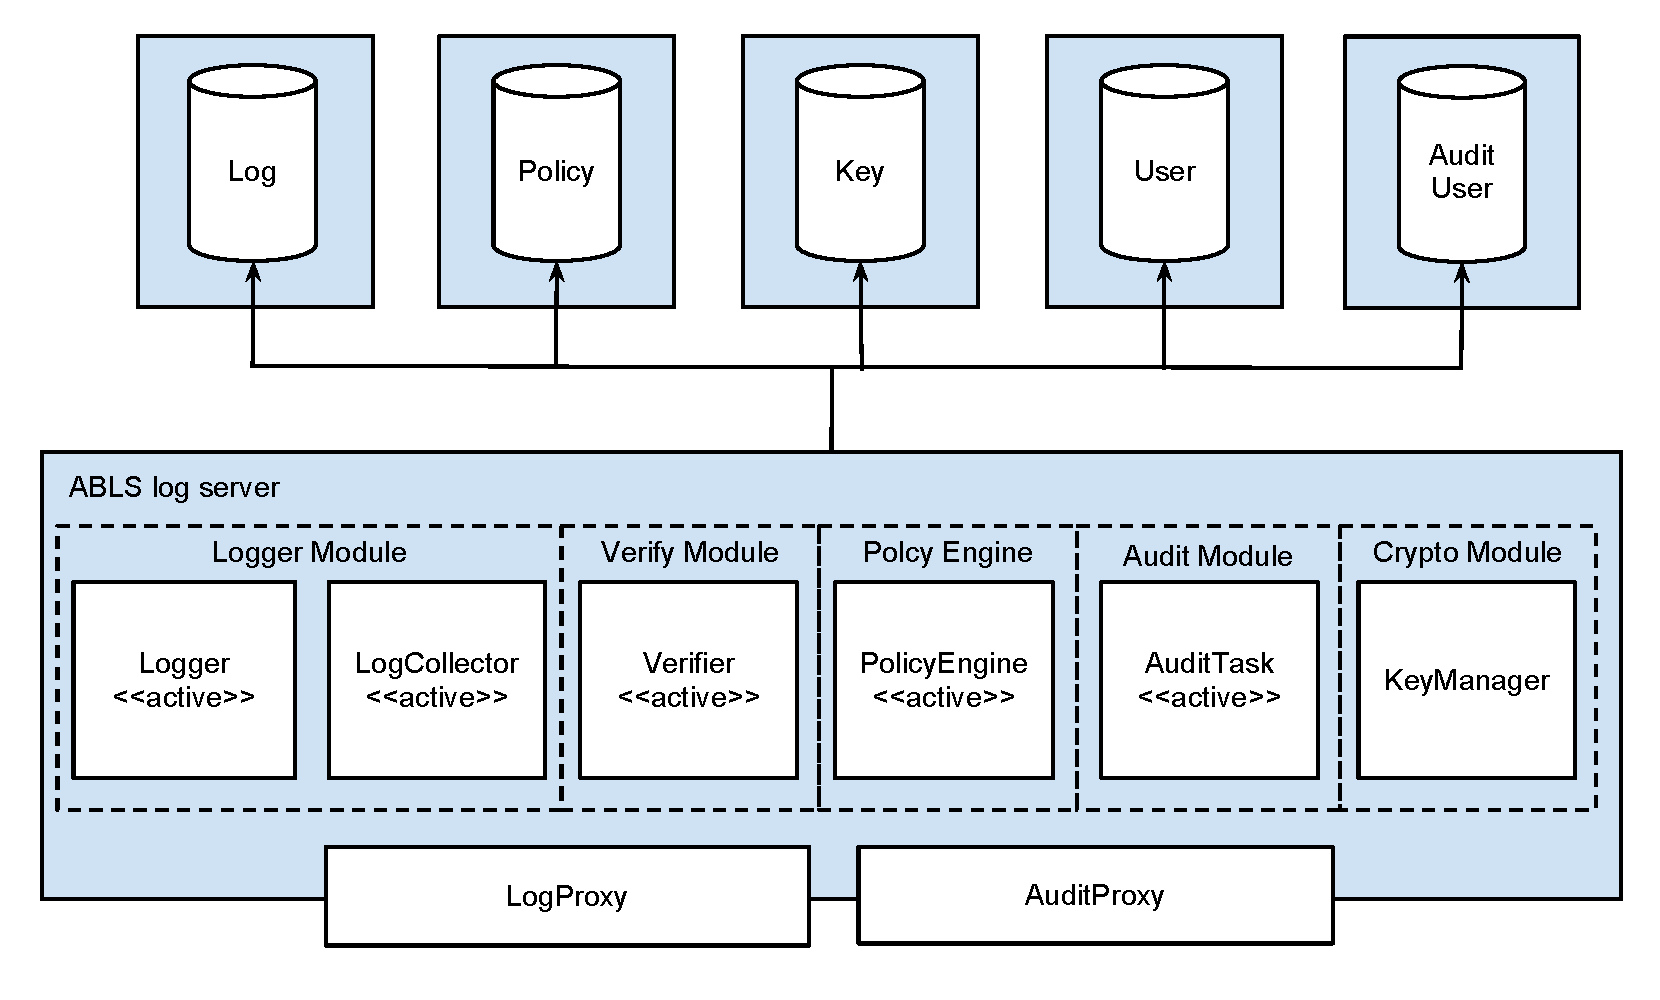
\includegraphics[width=4in]{images/deployment.pdf}
\caption{A high-level depiction of the deployment for an ABLS instance, where each box represents a unique runtime environment (i.e. a unique server).}
\label{fig:deployment}
\end{center}
\end{figure*}

Based on the purpose of each piece of data used in the log, it is best to physically separate databases
that store data of different security classes rather than rely on a single, segregated database that uses MAC with 
polyinstantiation to protect data of different security classes. Of course, access control
and authentication mechanisms for all of the database servers is enforced at the operating system level, thus
prohibiting immediate access to all unauthorized users other than the internal tasks (i.e. logger, verifier, policy engine, etc) 
within an ABLS instance. 

In the current ABLS prototype, all database servers are separated as individual SQLite database files. Once
the deployment platform is selected and properly configured, these will be replaced with instances of MySQL 
databases running on separate servers.

\subsection{Hybrid Key Management}
\label{sec:keyMgmt}

%TODO: expand with key manager object shared among everyone

In order to increase the performance of log entry encryption during a given user session, symmetric-key encryption
using AES-256 was chosen to encrypt all log entry messages. The symmetric key is then encrypted using the CP-ABE
scheme and persisted to the appropriate database. This design enhancement enables increased throughput
without sacrificing the level of confidentiality granularity that is needed for each log entry. However, should an 
unencrypted policy key for a given user's session become compromised, the remaining entries in that log database
are at risk of being compromised. 

The basic procedure for encrypting a log entry is shown in Algorithm \ref{alg:encrypt}. Once encrypted, the ciphertext
is stored in the database with the rest of the information necessary to continue the log chain for a given user's session.
  
\begin{algorithm}[ht!] %[htb]
\caption{Log entry encryption} \label{alg:encrypt}
\begin{algorithmic}[1]
\REQUIRE{An unencrypted log entry $L_i$ for session $S_j$ of user $U_k$}
% \ENSURE{The number of all minimum $(s,t)$-cuts of $G$}

% I decided not to list the input/output in this case, so that's why the above two lines are commented out
\STATE{Let $P$ be the access control policy for the message of $L_i$, as determined by the {\tt PolicyEngine}}
\IF{The symmetric key $K$ for $(U_k, S_j)$ has not been generated for $P$}
	\STATE{Generate $K$ and encrypt it with the CP-ABE encryption module using $P$, yielding $K_E$}
	\STATE{Persist $K_E$ to the key database}
\ELSE
	\STATE{Query the database for $K_E$, the encrypted key for policy $P$.}
	\STATE{Decrypt $K_E$ using the attributes of user $U_k$, yielding $K$}
\ENDIF
\STATE{Encrypt $L_i$ with AES-256 using $K$, yielding $E(L_i, K)$}
\STATE{Persist $E(L_i, K)$ to the log database}
\end{algorithmic}
\end{algorithm}

\subsection{Database Design}
\label{sec:databaseDesign}

%TODO: update with hashes, not encrypted data... 

As shown in section \ref{sec:deployment}, there are four main databases that must be maintained by ABLS:
the log, key, user, and policy database. The log database maintains all information in the log chain for every 
single user and session pair. The key database stores the cryptographic keys that were used to construct
such log chains. The user and policy databases store user information and policy rules for ABLS, respectively. 
In the current prototype of ABLS, the policy database is not used internally. Instead, all event rules are 
hard-coded into the {\tt PolicyEngine}. 

In order to link the entries in the log tables to their corresponding verification and encryption keys in the key database,
common user and session IDs are used (though not as the primary key for the tables since they do not satisfy
the uniqueness property). However, because such user and session information is stored in plaintext, their 
existence may lead to a violation of user privacy. Therefore, using a technique similar to the ``onion encryption'' design in
CryptDB \cite{Popa2012-CryptDB}, this information is now deterministically masked before being stored in the database.

This masking procedure works by encrypting the user and session attributes with a symmetric key generated
by the logger's master key salted by the user's unique identifier and target table identifier. In mathematical
terms, the encrypted user and session IDs, $[U_i]$ and $[S_j]$, stored in table $T$ are generated as follows.
\begin{align*}
[U_i] = E(M_k || H(U_i) || H(T), U_i) \\
[S_j] = E(M_k || H(U_i) || H(T), S_j) \\
\end{align*}

In this context, $M_k$ is the master key for the logger. Using the user and table identifiers as salts to the master key 
enable ensures that tables do not share any common information about the user, which helps prevent against 
inference attacks in the event that the database servers are compromised.

\subsection{Log Audits}
\label{sec:audit}
TODO: log query through audit protocol (users are stored in database, must login, can ask for data, and its formatted and returned to them)

\section{Completed Work}
For Phase 1 of the project, I focused mainly on fixing some of the design and implementation flaws in my previous 
prototype, redesigning the database to support the newly implemented symmetric key management scheme and data 
partitioning for different security classes, specifying the deployment scheme, and improving the quality test
of my internal unit tests and the functionality of the test driver program. The specifics of each of these improvements is
outlined in the following sections.

\subsection{Hybrid Key Management}
As described in Section \ref{sec:keyMgmt}, the process of encryption log messages was changed to use symmetric-key
encryption instead of CP-ABE due to the added performance improvement. Pairing-based cryptography is computationally
expensive, and under the assumption that ABLS might be subject to very heavy traffic loads at any particular time, the 
overhead of encrypting data to be stored in the database should be as minimal as possible. Therefore, each unique
policy that is needed to encrypt a log message is associated with a symmetric key, which is in turn encrypted using 
CP-ABE and then serialized to be stored in the key database. The Charm crypto package allows all cryptographic 
objects (which tend to be nested Python dictionaries and other complicated data structures) to be serialized to byte 
representations for database persistence. 

Also, in order to improve the performance of the logger, the per-policy symmetric keys for a user session are kept
in memory until the session has been closed. This avoids the need for the logger to query the database for the key 
when a new piece of data to be inserted into the log. 

Unfortunately, with this new key management scheme, the verification procedure becomes dependent on the
logger's master key. Thus, in order to support the verifiers, I started implementing a mechanism to share this key 
between them and the logger. I expect to complete this modification in Phase 2 of the project.

\subsection{Relational Database Design}
The relational database design was modified in order to support the new symmetric key management scheme and provide 
enhanced security for the stored data. In particular, rather than storing the cryptographic keys in the same database as the
log information, these two databases are now segregated and are expected to be deployed on different database servers.
By hardening both databases, a malicious attacker would now need to circumvent the access control 
mechanisms protecting two physically disjoint databases, rather than just one, in order to recover log 
decrypted messages. In terms of the actual implementation, this change caused many cascading errors 
throughout the code base which needed to be fixed before development continued.

Also, to better support audits that use the log database, a timestamp field was added to each table as a required
attribute. Not only does such information capture the exact timing of critical system events, it acts as a protection
mechanism in the event that log messages are inserted into the database out of order. Also, it is important to note that
each and every timestamp for a log message is generated as soon as the client handler reads the data from
its open socket. This is done to provide the most accurate timing information.

%Redesigned the relational database model to account for the different security classes among data that is used by ABLS. This resulted in a physical separation of database servers.
%TODO: added times, separated the database tables, optimized data types for columns to match what's stored

\subsection{Database Column Masking}
The initial implementation of the database masking procedure, which is outlined in Section \ref{sec:databaseDesign}
was started in this phase of the project. Currently, the ability for the logger to store the encrypted user and session IDs 
is not fully supported (only pseudocode has been written). In addition, the verifiers have yet to be updated to use 
this encrypted data to perform the strong verification check. This will finished in the next phase of the project.

\subsection{Bootstrapping, Test Enhancement, and Deployment}
In order to streamline the test and deployment phases of development, a bootstrap script was implemented to configure
new (empty) versions of the local SQLite databases. The main executable script (main.py) was also modified to support
development and production modes of operation, in which the development mode clears the contents of every 
database and then proceeds to insert false user data into the users table to begin the logging process. The test 
driver program, TrafficProxyDriver.py, was then modified accordingly to use the default data contained within the 
database. With these changes, the typical process to start and interact with an ABLS instance is as follows.

\begin{enumerate}
	\item Run the bootstrap script to create new versions of the local SQLite databases. In the actual deployment of an ABLS instance, this script would connect to the remote databases and specify their schemas accordingly. Thus, it is meant only for development purposes and should not be used on a live ABLS instance.
	\item Run the main executable file (main.py) with the -c (configure) to flag to enable development mode, in which the databases are wiped clean and replaced with a small set of fake data. If one wishes to start an ABLS instance at this point in time, they may also add the -s (start) flag to the script so that it starts the ABLS instance.
	\item Run the test driver program (TrafficProxyDriver.py) and point it to the host and port at which the traffic proxy within the ABLS instance is listening. By default, these are ``localhost'' and port 9998, but they can easily be changed to any other values in the source code. 
\end{enumerate}

Aside from the initialization code, the test driver program now includes a more robust suite of tests to simulate varying traffic 
loads. The user interface of this program was also improved so as to aid the developers in interacting with the ABLS 
prototype at runtime. Given the difficulty of testing this distributed system at runtime, creating a more sophisticated
test driver was crucial to the development process that enabled smoke tests to be run with minimal effort.

However, despite the increased complexity of the test driver, it does not, nor will it ever, support the ability to acquire 
diagnostic information from the ABLS runtime. This information is logged by the ABLS instances to the appropriate log 
file, and the administrators for the ABLS system can check this information at their discretion.

\subsection{Outstanding Bug Fixes}
As a result of resuming my work from the previous quarter, some of my time spent during Phase 1 was devoted to fixing
outstanding design and performance bugs in the ABLS prototype. Some of the notable bugs include improper 
initialization of the verifier threads and incorrect management of the in-memory data structures containing the 
user session information (i.e. data specific to the generation of log messages).

\subsection{Research and Literature Survey}
An initial action item for this work was to investigate the possibility of replacing the relational database model with a 
NoSQL model. I spent a significant amount of time during week 4 investigating the benefits of making a transition
to such a DBMS. In particular, I examined MongoDB, a common document-based NoSQL database. Unfortunately,
my research revealed that MongoDB is not an ACID system, and thus transactions are not guaranteed to keep the
database in a consistent state. In the context of ABLS, a failed transaction could put the system in a bad state. Therefore,
I made the decision to keep the relational database model but hide the user-sensitive information using the techniques
discussed in Section \ref{sec:databaseDesign}.

A comprehensive literature survey on related logging and non-repudiation work was also completed during this phase 
of the project. The corresponding articles that were read are included in this phase's submission package. The digest 
of this work is expected to be a part of the final paper.

\subsection{Log Traffic Encryption}
The ABLS prototype now supports SSL encryption of all incoming log traffic to ensure the confidentiality of sensitive
information as it is sent from the client to the server running the traffic proxy. Unfortunately, this is only one-way SSL 
authentication in which the client verifies the server. I am currently experimenting with ways to implement two-way 
SSL authentication so the client can be verified as well, which is the ultimate goal. 

\subsection{Log Collection}
As part of the proposed design, all log messages generated by the logger to be inserted into the 
database will be handed off to a common log collector to do so. This log collector will be implemented as a 
separate actor (thread) running within the ABLS process and will assume a portion of the database 
communication overhead from the logger to free up cycles for processing more log messages. Each logger instance
will point to the same log collector thread or log collector pool, if needed to increase the throughput of database 
transactions. Furthermore, all log collector tasks will be spawned when the ABLS instance first loads.

\subsection{Complete Database Masking}
Following the design outlined in Section \ref{sec:databaseDesign}, the database masking scheme will be completed by
adding support to the database verifiers. Since the verifiers run within the context of the ABLS system, they will be granted
permission to all of the database servers. This will enable them to request the appropriate entity and epoch keys 
needed to perform strong verification checks on the data in user session log chains. Also, this must be the first 
activity that is completed because the log querying and automated audit tasks depend on the database columns 
being properly masked. 

\subsection{Log Querying}
\label{sec:querying}
In order to make ABLS fulfill its purpose as a secure logging system, log query support will be added to the audit
module. Such query support will be exposed to clients through a lightweight API that is used via the audit protocol.
To start, only select operations parameterized by the user ID or both the user and session IDs will be supported. 
As an example, the API might have the following function signatures. \\

\noindent {\tt selectByUser(int uid)} \\
{\tt selectByUserAndSession(int uid, int sid)}\\

Clients will connect to the audit proxy, which is similar to the log traffic proxy, and issue commands according to
the audit protocol to invoke either one of these functions. Client authentication is expected to be completed at a later
point in time as outlined in Section \ref{sec:auth}. Assuming the client has been authenticated, they can issue commands
wrapped in JSON strings with the following format to the audit proxy. \\

\begin{lstlisting}
{     
    "command" : command_id
    "params" : csv_list
}
\end{lstlisting}

Upon receiving and parsing an incoming command, the client handler, which is spawned to handle each client connection,
will issue the appropriate command to the log module to select the appropriate log message contents from the database. 
However, since each client is expected to be a user for the ABLS instance, their attributes will be used to filter 
the resulting database rows that are returned. Thus, the audit proxy and client handlers will act
as a reference monitor that enforces access control to the log database through the log query protocol and API.

In order to implement this action item, I will complete the following tasks.

\begin{enumerate}
	\item Implement the audit proxy with a corresponding client handler thread using the same technique that was done for the traffic proxy. 
	\item Implement the functionality in the client handlers to parse messages according to the log query protocol.
	\item Implement the functionality to collate log message for the specific query in a temporary location.
	\item Using the client's attributes, filter all messages that cannot be decrypted according to the embedded ciphertext policy.
	\item Format the results in a JSON string that is sent back to the client.
\end{enumerate}

Unlike the traffic proxy, it is expected that the clients for the audit proxy will be authenticated using passwords. Thus, as
part of supporting client authentication, a proper password storage scheme will need to be implemented, which includes 
the modification of the user database schema and proper password hashing (and salting) techniques. 

\subsection{ABLS Configuration File} 
In order to improve the quality of the ABLS prototype, all of the hard-coded configuration strings that set up databases,
specify cryptographic certificate locations, and log file output directories will be removed and placed in a configuration file
to be managed by system administrators. Access to this file will be restricted to system administrators and enforced by the 
operating system. An example of how the configuration file might look is shown below.

\begin{lstlisting}
# comment
log_database: network location string
key_database: network location string
user_database: network location string
log_file: absolute path string
...
\end{lstlisting}

\section{Future Work}
For the remainder of the project I plan to finish up the outstanding tasks mentioned in the previous section and 
focus mainly on the auditing aspects of ABLS. Auditing will be supported both manually and automatically through
a robust log query interface, which places the ABLS runtime in the role of the log database reference monitor, and 
automated strategy-driven tasks run within the context of the ABLS runtime, respectively. The following 
sections expand upon all of these action items in more detail.

\subsection{Audit Strategy Design - 1/24/13}
As the number of contents in the log database grows, manual audits conducted by querying the log become less and less 
feasible. Therefore, the audit module will be extended with strategy-driven audit tasks that can scan the log database 
on-demand to check for policy violations. In order to enable clients to define these audit strategies, there must be a 
formal way of mapping security policies into log query strategies. For example, if one such policy is that no user should use 
the application between the hours of 12:00am and 6:00am, then the audit task must be able to interpret this information
and query the log database for messages stored in this time frame. 

Currently, the plan for implementing this mapping is to provide clients with a set of parameters that they can populate to
match their desired security policies. A subset of these parameters is shown below.
\begin{lstlisting}
eventId: event id
occurred_flag: flag for event occurrence
target_user: source user id
time_range: time range for the event
\end{lstlisting}

Of course, this information may also be encoded using EPAL or XACML \cite{Anderson2005-ComparisonEAPL_XACML}.
However, this homegrown mapping will be used to avoid the implementation of complex XML parsers. 

With this mapping in place, audit strategies will be developed in two phases. The first phase will enable the 
ABLS administrator to specify audit strategies before deploying an ABLS instance, at which point the strategies 
will be fixed. This will be done by manually modifying the audit task source code. The second phase will enable 
clients to dynamically configure audit strategies while an ABLS instance is currently running. This will be done 
by parsing client-provided JSON strings containing the aforementioned parameters. The audit protocol will also 
be updated to include a command to specify a new audit task strategy.

\subsection{Client Authentication - 1/31/13}
\label{sec:auth}
There are two types of clients that can interact with an ABLS instance at runtime: the clients generating log data and the
clients requesting log data (for the purpose of auditing). To support log message confidentiality, clients generating 
log data will be authenticated using two-way SSL authentication, as shown in Figure \ref{fig:ssl}. This will 
promote a bidirectional measure of trust between the client and server while at the same time encrypting 
all sensitive data as it is sent between the two endpoints. Also, without an appropriate certificate authority, all
of the certificates will be self-signed for verification purposes. Actual deployments will require these certificates
to be signed by a legitimate CA.

\begin{figure}[ht!]
\begin{center}
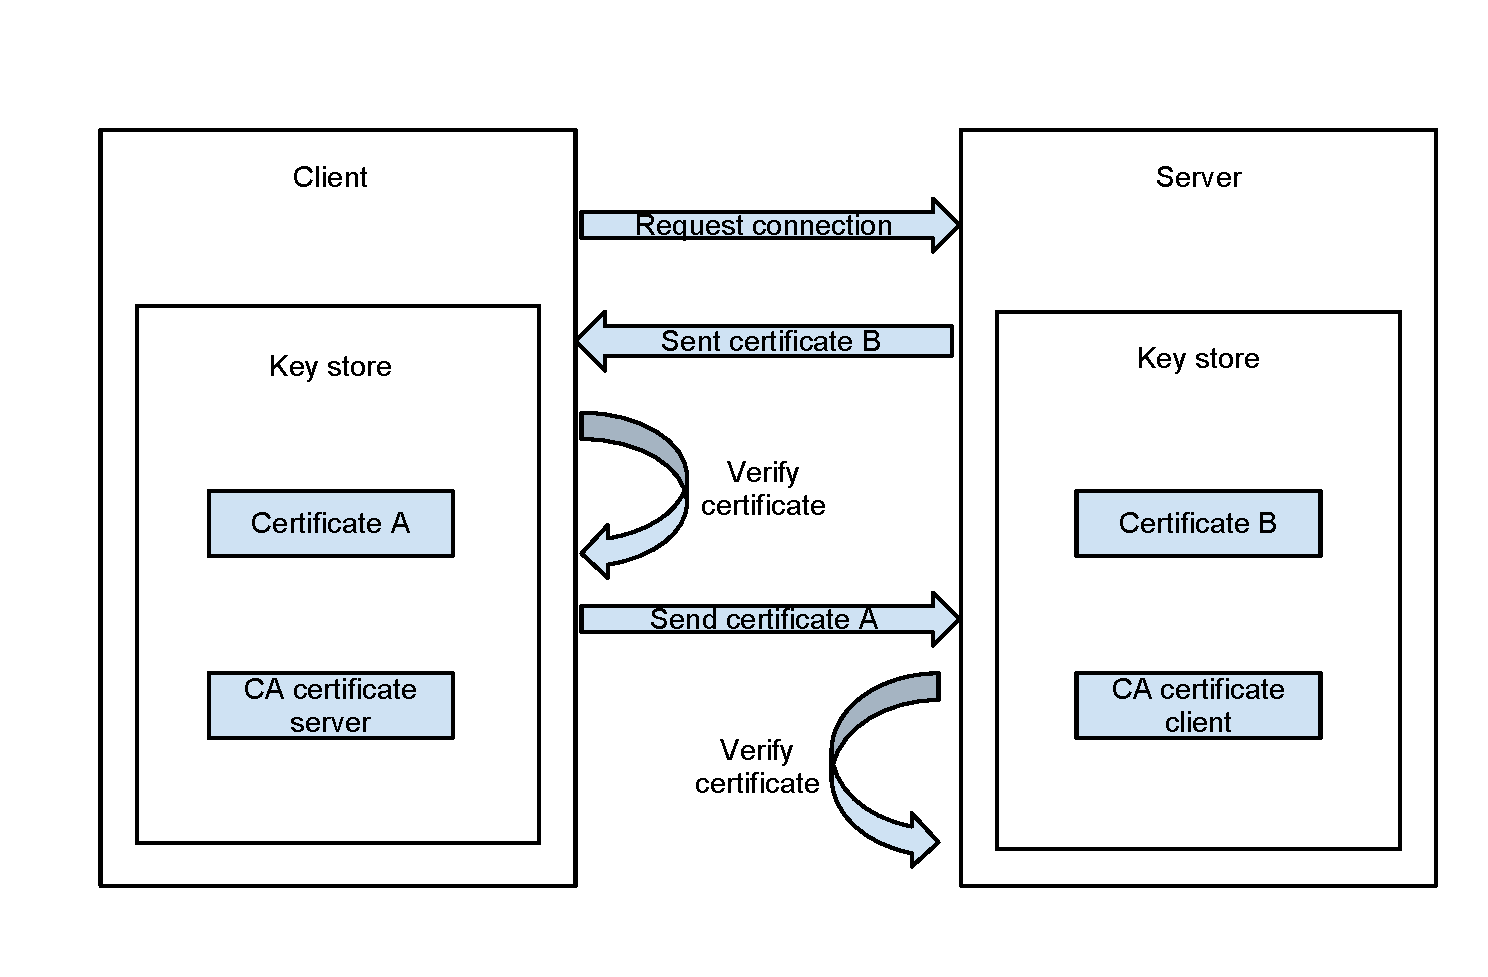
\includegraphics[width=3in]{images/two_way_ssl.pdf}
\caption{A pictorial representation of two-way SSL authentication. }
\label{fig:ssl}
\end{center}
\end{figure}

Authentication for the clients that request log data will be done with the use of passwords, similar in style to how the 
FTP protocol authenticates users. As discussed in Section \ref{sec:querying}, this will require the implementation of 
a secure password management scheme that uses the appropriate cryptographic techniques. 

%TODO: public-key authentication using SSL certificates (prefered), user logins for audit interface

\section{Attack Strategy}
\label{sec:attack}

TODO: combination of static/dynamic automated and manual tests (look for config and code errors)

Appscan for the web app, Nessus and metasploit for the server and then some database specific tool to check for default configs and shit

\begin{comment}
\begin{table}
\centering
\caption{Feelings about Issues}
\begin{tabular}{|l|r|l|} \hline
Flavor&Percentage&Comments\\ \hline
Issue 1 &  10\% & Loved it a lot\\ \hline
Issue 2 &  20\% & Disliked it immensely\\ \hline
Issue 3 &  30\% & Didn't care one bit\\ \hline
Issue 4 &  40\% & Duh?\\ \hline
\end{tabular}
\end{table}

\begin{figure}[ht!]
\label{sample graphic}
\begin{center}
\includegraphics[width=1.5in]{fly.jpg}
\caption{A sample black \& white graphic (JPG).}
\end{center}
\end{figure}
\end{comment}

\bibliographystyle{abbrv}
\bibliography{../abls}
% You must have a proper ".bib" file
%  and remember to run:
% latex bibtex latex latex
% to resolve all references
\balance
\end{document}
